\documentclass{standalone}
\usepackage{tikz}
\usetikzlibrary{patterns, positioning}
\usepackage[sfdefault]{ClearSans} %% option 'sfdefault' activates Clear Sans as the default text font
\usepackage[T1]{fontenc}

\begin{document}
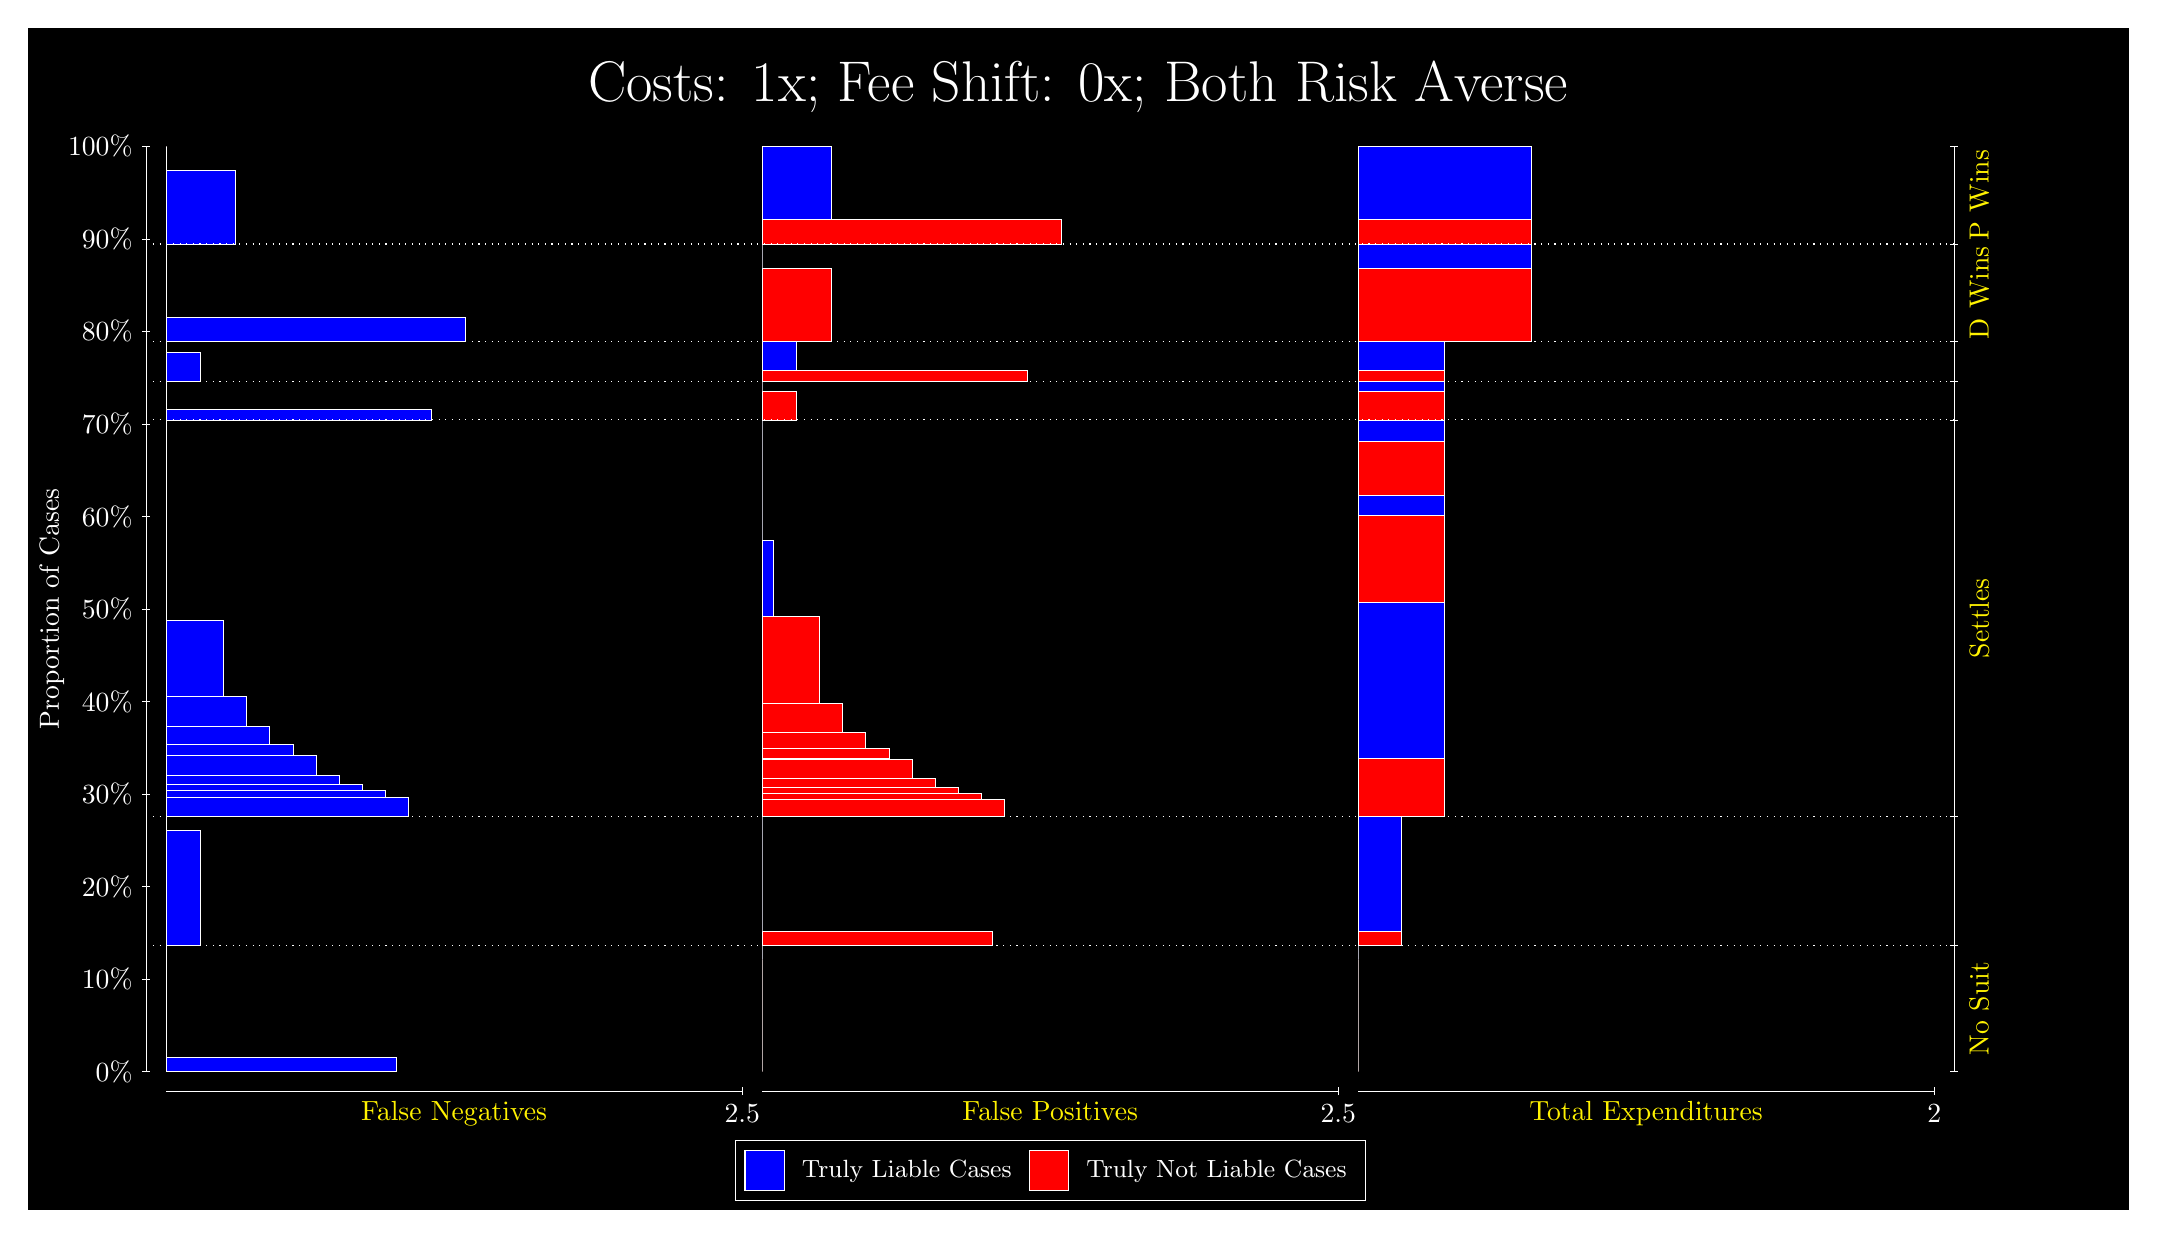
\begin{tikzpicture}
\draw[fill=black] (0,0) rectangle (26.667,15);
\draw[text=white] (0,13.5) rectangle (26.667,15) node[midway] {\huge Costs: 1x; Fee Shift: 0x; Both Risk Averse};
\draw[white, very thin] (1.5,1.75) -- (1.5,13.5);
\node[rotate=90, text=white, anchor=center] at (0.3, 7.625) {Proportion of Cases};
\draw[white, very thin] (1.45,1.75) -- (1.55,1.75);
\node[text=white, anchor=east] at (1.45, 1.75) {0\%};
\draw[white, very thin] (1.45,2.925) -- (1.55,2.925);
\node[text=white, anchor=east] at (1.45, 2.925) {10\%};
\draw[white, very thin] (1.45,4.1) -- (1.55,4.1);
\node[text=white, anchor=east] at (1.45, 4.1) {20\%};
\draw[white, very thin] (1.45,5.275) -- (1.55,5.275);
\node[text=white, anchor=east] at (1.45, 5.275) {30\%};
\draw[white, very thin] (1.45,6.45) -- (1.55,6.45);
\node[text=white, anchor=east] at (1.45, 6.45) {40\%};
\draw[white, very thin] (1.45,7.625) -- (1.55,7.625);
\node[text=white, anchor=east] at (1.45, 7.625) {50\%};
\draw[white, very thin] (1.45,8.8) -- (1.55,8.8);
\node[text=white, anchor=east] at (1.45, 8.8) {60\%};
\draw[white, very thin] (1.45,9.975) -- (1.55,9.975);
\node[text=white, anchor=east] at (1.45, 9.975) {70\%};
\draw[white, very thin] (1.45,11.15) -- (1.55,11.15);
\node[text=white, anchor=east] at (1.45, 11.15) {80\%};
\draw[white, very thin] (1.45,12.325) -- (1.55,12.325);
\node[text=white, anchor=east] at (1.45, 12.325) {90\%};
\draw[white, very thin] (1.45,13.5) -- (1.55,13.5);
\node[text=white, anchor=east] at (1.45, 13.5) {100\%};

\draw[white, very thin] (24.457,1.75) -- (24.457,13.5);
\draw[white, very thin] (24.407,1.75) -- (24.507,1.75);
\node[anchor=west] at (24.407, 1.75) {};
\draw[white, very thin] (24.407,3.3501) -- (24.507,3.3501);
\node[anchor=west] at (24.407, 3.3501) {};
\draw[white, very thin] (24.407,4.9869) -- (24.507,4.9869);
\node[anchor=west] at (24.407, 4.9869) {};
\draw[white, very thin] (24.407,10.026) -- (24.507,10.026);
\node[anchor=west] at (24.407, 10.026) {};
\draw[white, very thin] (24.407,10.517) -- (24.507,10.517);
\node[anchor=west] at (24.407, 10.517) {};
\draw[white, very thin] (24.407,11.022) -- (24.507,11.022);
\node[anchor=west] at (24.407, 11.022) {};
\draw[white, very thin] (24.407,12.26) -- (24.507,12.26);
\node[anchor=west] at (24.407, 12.26) {};
\draw[white, very thin] (24.407,13.5) -- (24.507,13.5);
\node[anchor=west] at (24.407, 13.5) {};

\draw[white, very thin, fill=blue] (1.75,1.75) rectangle (4.6775,1.9256);
\draw[white, very thin, fill=red] (1.75,1.9256) rectangle (1.75,3.3501);
\draw[white, very thin, fill=blue] (1.75,3.3501) rectangle (2.1891,4.8114);
\draw[white, very thin, fill=red] (1.75,4.8114) rectangle (1.75,4.9869);
\draw[white, very thin, fill=blue] (1.75,4.9869) rectangle (4.8239,5.2367);
\draw[white, very thin, fill=blue] (1.75,5.2367) rectangle (4.5312,5.327);
\draw[white, very thin, fill=blue] (1.75,5.327) rectangle (4.2384,5.3967);
\draw[white, very thin, fill=blue] (1.75,5.3967) rectangle (3.9457,5.517);
\draw[white, very thin, fill=blue] (1.75,5.517) rectangle (3.6529,5.7693);
\draw[white, very thin, fill=blue] (1.75,5.7693) rectangle (3.3602,5.9);
\draw[white, very thin, fill=blue] (1.75,5.9) rectangle (3.0674,6.1342);
\draw[white, very thin, fill=blue] (1.75,6.1342) rectangle (2.7746,6.5111);
\draw[white, very thin, fill=blue] (1.75,6.5111) rectangle (2.4819,7.4846);
\draw[white, very thin, fill=red] (1.75,7.4846) rectangle (1.75,10.026);
\draw[white, very thin, fill=blue] (1.75,10.026) rectangle (5.1167,10.159);
\draw[white, very thin, fill=red] (1.75,10.159) rectangle (1.75,10.517);
\draw[white, very thin, fill=blue] (1.75,10.517) rectangle (2.1891,10.883);
\draw[white, very thin, fill=red] (1.75,10.883) rectangle (1.75,11.022);
\draw[white, very thin, fill=blue] (1.75,11.022) rectangle (5.5558,11.332);
\draw[white, very thin, fill=red] (1.75,11.332) rectangle (1.75,12.26);
\draw[white, very thin, fill=blue] (1.75,12.26) rectangle (2.6283,13.191);
\draw[white, very thin, fill=red] (1.75,13.191) rectangle (1.75,13.5);
\draw[white, very thin, fill=red] (9.3189,1.75) rectangle (9.3189,3.1745);
\draw[white, very thin, fill=blue] (9.3189,3.1745) rectangle (9.3189,3.3501);
\draw[white, very thin, fill=red] (9.3189,3.3501) rectangle (12.246,3.5256);
\draw[white, very thin, fill=blue] (9.3189,3.5256) rectangle (9.3189,4.9869);
\draw[white, very thin, fill=red] (9.3189,4.9869) rectangle (12.393,5.2014);
\draw[white, very thin, fill=red] (9.3189,5.2014) rectangle (12.1,5.2897);
\draw[white, very thin, fill=red] (9.3189,5.2897) rectangle (11.807,5.3619);
\draw[white, very thin, fill=red] (9.3189,5.3619) rectangle (11.515,5.4687);
\draw[white, very thin, fill=red] (9.3189,5.4687) rectangle (11.222,5.7151);
\draw[white, very thin, fill=red] (9.3189,5.7151) rectangle (10.929,5.7287);
\draw[white, very thin, fill=red] (9.3189,5.7287) rectangle (10.929,5.8559);
\draw[white, very thin, fill=red] (9.3189,5.8559) rectangle (10.636,6.0622);
\draw[white, very thin, fill=red] (9.3189,6.0622) rectangle (10.344,6.4215);
\draw[white, very thin, fill=red] (9.3189,6.4215) rectangle (10.051,7.5282);
\draw[white, very thin, fill=blue] (9.3189,7.5282) rectangle (9.4652,8.5017);
\draw[white, very thin, fill=blue] (9.3189,8.5017) rectangle (9.3189,10.026);
\draw[white, very thin, fill=red] (9.3189,10.026) rectangle (9.758,10.383);
\draw[white, very thin, fill=blue] (9.3189,10.383) rectangle (9.3189,10.517);
\draw[white, very thin, fill=red] (9.3189,10.517) rectangle (12.686,10.655);
\draw[white, very thin, fill=blue] (9.3189,10.655) rectangle (9.758,11.022);
\draw[white, very thin, fill=red] (9.3189,11.022) rectangle (10.197,11.95);
\draw[white, very thin, fill=blue] (9.3189,11.95) rectangle (9.3189,12.26);
\draw[white, very thin, fill=red] (9.3189,12.26) rectangle (13.125,12.569);
\draw[white, very thin, fill=blue] (9.3189,12.569) rectangle (10.197,13.5);
\draw[white, very thin, fill=red] (16.888,1.75) rectangle (16.888,3.1745);
\draw[white, very thin, fill=blue] (16.888,3.1745) rectangle (16.888,3.3501);
\draw[white, very thin, fill=red] (16.888,3.3501) rectangle (17.437,3.5256);
\draw[white, very thin, fill=blue] (16.888,3.5256) rectangle (17.437,4.9869);
\draw[white, very thin, fill=red] (16.888,4.9869) rectangle (17.986,5.7287);
\draw[white, very thin, fill=blue] (16.888,5.7287) rectangle (17.986,7.7082);
\draw[white, very thin, fill=red] (16.888,7.7082) rectangle (17.986,8.8149);
\draw[white, very thin, fill=blue] (16.888,8.8149) rectangle (17.986,9.0647);
\draw[white, very thin, fill=red] (16.888,9.0647) rectangle (17.986,9.7575);
\draw[white, very thin, fill=blue] (16.888,9.7575) rectangle (17.986,10.026);
\draw[white, very thin, fill=red] (16.888,10.026) rectangle (17.986,10.383);
\draw[white, very thin, fill=blue] (16.888,10.383) rectangle (17.986,10.517);
\draw[white, very thin, fill=red] (16.888,10.517) rectangle (17.986,10.655);
\draw[white, very thin, fill=blue] (16.888,10.655) rectangle (17.986,11.022);
\draw[white, very thin, fill=red] (16.888,11.022) rectangle (19.083,11.95);
\draw[white, very thin, fill=blue] (16.888,11.95) rectangle (19.083,12.26);
\draw[white, very thin, fill=red] (16.888,12.26) rectangle (19.083,12.569);
\draw[white, very thin, fill=blue] (16.888,12.569) rectangle (19.083,13.5);
\draw[white, dotted] (1.5,3.3501) -- (24.457,3.3501);
\draw[white, dotted] (1.5,4.9869) -- (24.457,4.9869);
\draw[white, dotted] (1.5,10.026) -- (24.457,10.026);
\draw[white, dotted] (1.5,10.517) -- (24.457,10.517);
\draw[white, dotted] (1.5,11.022) -- (24.457,11.022);
\draw[white, dotted] (1.5,12.26) -- (24.457,12.26);
\draw[white, very thin] (1.75,1.5) -- (9.0689,1.5);
\node[text=yellow, anchor=north] at (5.4094, 1.5) {False Negatives};
\draw[white, very thin] (9.0689,1.45) -- (9.0689,1.55);
\node[text=white, anchor=north] at (9.0689, 1.45) {2.5};

\draw[white, very thin] (9.3189,1.5) -- (16.638,1.5);
\node[text=yellow, anchor=north] at (12.978, 1.5) {False Positives};
\draw[white, very thin] (16.638,1.45) -- (16.638,1.55);
\node[text=white, anchor=north] at (16.638, 1.45) {2.5};

\draw[white, very thin] (16.888,1.5) -- (24.207,1.5);
\node[text=yellow, anchor=north] at (20.547, 1.5) {Total Expenditures};
\draw[white, very thin] (24.207,1.45) -- (24.207,1.55);
\node[text=white, anchor=north] at (24.207, 1.45) {2};

\node[text=yellow, centered, rotate=90] at (24.777, 2.55) {No Suit};

\node[text=yellow, centered, rotate=90] at (24.777, 7.5064) {Settles};


\node[text=yellow, centered, rotate=90] at (24.777, 11.641) {D Wins};
\node[text=yellow, centered, rotate=90] at (24.777, 12.88) {P Wins};

\draw (12.978300999999998,1.5) node[draw=none] (baseCoordinate) {};
\begin{scope}[align=center]
        \matrix[scale=0.5, draw=white, below=0.5cm of baseCoordinate, nodes={draw}, column sep=0.1cm]{
            \node[rectangle, draw, minimum width=0.5cm, minimum height=0.5cm, fill=blue] {}; &
            \node[draw=none, font=\small, text=white] (B) {Truly Liable Cases}; &
            \node[rectangle, draw, minimum width=0.5cm, minimum height=0.5cm, fill=red] {}; &
            \node[draw=none, font=\small, text=white] (B) {Truly Not Liable Cases}; \\
            };
\end{scope}

\end{tikzpicture}
\end{document}